\documentclass[varwidth=40cm]{standalone}
\usepackage{tikz}
\usepackage{pgfplots}
\usepackage{style}

\begin{document}
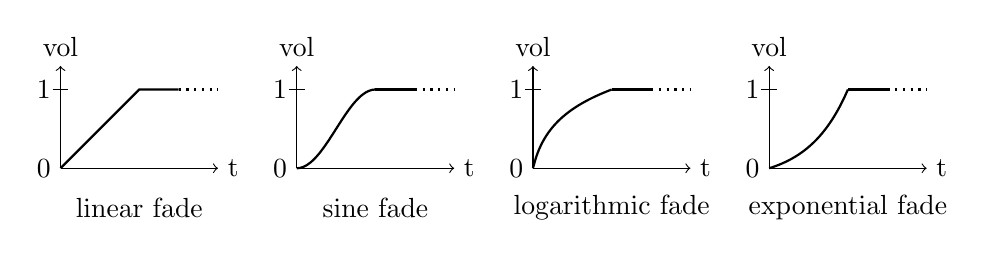
\begin{tikzpicture}
  \draw[->] (0,0) -- (2,0) node[right] {t};
  \draw[->] (0,0) -- (0,1.3) node[above] {vol};
  \draw (-.1,1) -- (.1,1);
  \draw (0,0) node[left] {0};
  \draw (0,1) node[left] {1};
  \draw[thick] (0,0) -- (1,1) -- (1.5,1);
  \draw[thick,dotted] (1.5,1) -- (2,1);
  \draw(1,-.5) node {linear fade};

  \begin{scope}[shift={(3,0)}]
    \draw[->] (0,0) -- (2,0) node[right] {t};
    \draw[->] (0,0) -- (0,1.3) node[above] {vol};
    \draw (-.1,1) -- (.1,1);
    \draw (0,0) node[left] {0};
    \draw (0,1) node[left] {1};
    \draw[domain=0:1, smooth, thick, variable=\x] plot ({\x}, {(1+sin((\x-0.5)*180))/2});
    \draw[thick] (1,1) -- (1.5,1);
    \draw[thick,dotted] (1.5,1) -- (2,1);
    \draw(1,-.5) node {sine fade};
  \end{scope}

  \begin{scope}[shift={(6,0)}]
    \draw[->] (0,0) -- (2,0) node[right] {t};
    \draw[->] (0,0) -- (0,1.3) node[above] {vol};
    \draw (-.1,1) -- (.1,1);
    \draw (0,0) node[left] {0};
    \draw (0,1) node[left] {1};
    \draw[domain=0:1, smooth, thick, variable=\x] plot ({\x}, {ln(1+10*\x)/ln(1+10)});
    \draw[thick] (1,1) -- (1.5,1);
    \draw[thick,dotted] (1.5,1) -- (2,1);
    \draw(1,-.5) node {logarithmic fade};    
  \end{scope}
  
  \begin{scope}[shift={(9,0)}]
    \draw[->] (0,0) -- (2,0) node[right] {t};
    \draw[->] (0,0) -- (0,1.3) node[above] {vol};
    \draw (-.1,1) -- (.1,1);
    \draw (0,0) node[left] {0};
    \draw (0,1) node[left] {1};
    \draw[domain=0:1, smooth, thick, variable=\x] plot ({\x}, {(exp(2*\x-1)-exp(-1))/(exp(2-1)-exp(-1))});
    \draw[thick] (1,1) -- (1.5,1);
    \draw[thick,dotted] (1.5,1) -- (2,1);
    \draw(1,-.5) node {exponential fade};
  \end{scope}
\end{tikzpicture}
\end{document}
